\documentclass[a4paper,12pt]{article}
\usepackage{a4wide}
\usepackage{tikz}
\usetikzlibrary{calc}
\usepackage{hyperref}

\begin{document}
\pagestyle{empty}
\setlength{\parindent}{0em} 
\section*{CRC (Cyclic Redundancy Check)}
Your task is to program the behavior of an entity called "crc". This entity is declared in the attached file "crc.vhdl" and has the following properties:

\begin{itemize}
\item Input: NEW\_MSG of type std\_logic
\item Input: MSG of type std\_logic\_vector with length %%MSGLEN 
\item Input: CLK of type std\_logic
\item Output: CRC of std\_logic\_vector with length %%GENDEG
\item Output: CRC\_VALID of type std\_logic
\end{itemize}

\vspace{0.5cm}

\begin{center}
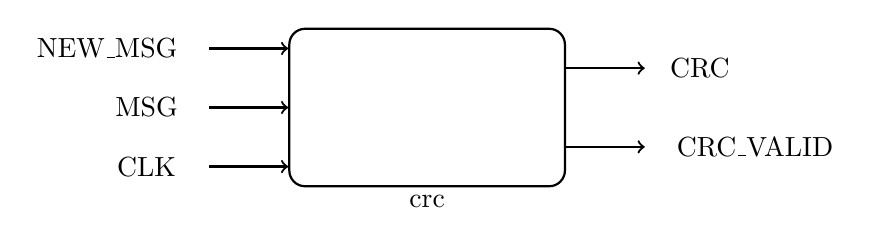
\begin{tikzpicture}
\draw node [draw,rectangle, minimum height=20mm, minimum width=35mm,rounded corners=2mm,thick](entity){};

\draw[->,thick] ($ (entity.west)+(-10mm,7.5mm) $) -- ($ (entity.west) +(0mm,7.5mm)$);
\draw node at ($ (entity.west)+(-23mm,7.5mm) $){NEW\_MSG};

\draw[->,thick] ($ (entity.west)+(-10mm,0mm) $) -- ($ (entity.west) +(0mm,0mm)$);
\draw node at ($ (entity.west)+(-18mm,0mm) $){MSG};

\draw[->,thick] ($ (entity.west)+(-10mm,-7.5mm) $) -- ($ (entity.west) + (0mm,-7.5mm)$);
\draw node at ($ (entity.west)+(-18mm,-7.5mm) $){CLK};

\draw[->,thick] ($(entity.east)+(0mm,+5mm) $) -- ($(entity.east)+(+10mm,+5mm)$);
\draw node at ($ (entity.east) + (17mm,+5mm) $){CRC};

\draw[->,thick] ($(entity.east)+(0mm,-5mm) $) -- ($(entity.east)+(+10mm,-5mm)$);
\draw node at ($ (entity.east) + (24mm,-5mm)$){CRC\_VALID};

\draw node at ($ (entity) - (0,12mm)$){crc};

\end{tikzpicture}
\end{center}

Do not change the file "crc.vhdl".
\\

The "crc" entity shall generate a crc for a message with the following constraints:
\begin{itemize}
\item Message length: %%MSGLEN
\item Generator degree: %%GENDEG
\item Generator polynomial: $%%GENSTRING$ (%%GENBIN)
\end{itemize}
The process of calculation follows the following scheme:
\begin{enumerate}
    \item A rising edge at port NEW\_MSG indicates a new CRC calculation for the message at port MSG has to be performed.
    \item After %%CLOCKCYCLES clock cycles of the clock at port CLK the calculated CRC has to be set at port CRC and the port CRC\_VALID has to be set to 1 to indicate a valid calculation result.
\end{enumerate}

\newpage

To calculate the CRC the entity "crc" shall use a feedback shift register "fsr". This entity is declared in the attached file "fsr.vhdl" and has the following properties:
\begin{itemize}
    \item Input: EN of type std\_logic
    \item Input: RST of type std\_logic 
    \item Input: CLK of type std\_logic
    \item Input: DATA\_IN of type std\_logic
    \item Output: DATA of type std\_logic\_vector with length %%CRCWIDTH
\end{itemize}

\vspace{0.5cm}

\begin{center}
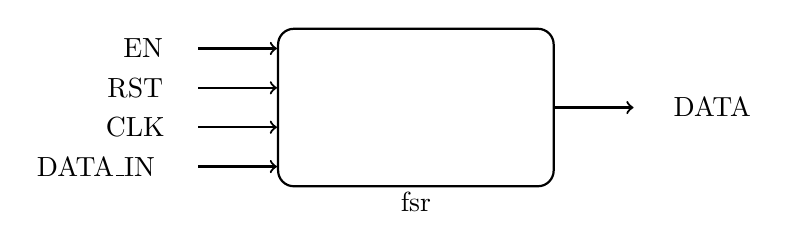
\begin{tikzpicture}
\draw node [draw,rectangle, minimum height=20mm, minimum width=35mm,rounded corners=2mm,thick](entity){};

\draw[->,thick] ($ (entity.west)+(-10mm,7.5mm) $) -- ($ (entity.west) +(0mm,7.5mm)$);
\draw node at ($ (entity.west)+(-17mm,7.5mm) $){EN};

\draw[->,thick] ($ (entity.west)+(-10mm,2.5mm) $) -- ($ (entity.west) +(0mm,2.5mm)$);
\draw node at ($ (entity.west)+(-18mm,2.5mm) $){RST};

\draw[->,thick] ($ (entity.west)+(-10mm,-2.5mm) $) -- ($ (entity.west) +(0mm,-2.5mm)$);
\draw node at ($ (entity.west)+(-18mm,-2.5mm) $){CLK};

\draw[->,thick] ($ (entity.west)+(-10mm,-7.5mm) $) -- ($ (entity.west) + (0mm,-7.5mm)$);
\draw node at ($ (entity.west)+(-23mm,-7.5mm) $){DATA\_IN};

\draw[->,thick] ($(entity.east)+(0mm,+0mm) $) -- ($(entity.east)+(+10mm,+0mm)$);
\draw node at ($ (entity.east) + (20mm,+0mm) $){DATA};

\draw node at ($ (entity) - (0,12mm)$){fsr};

\end{tikzpicture}
\end{center}

Do not change the file "fsr.vhdl".
\\

The feedback shift register should have the following behavior: 
\begin{itemize}
    \item The fsr's activity is controlled by the active high enable port EN.
    \item A rising edge at port RST resets the content of the shift register to all 0.
    \item On each rising edge of CLK the shift and feedback operation is done with the bit at port DATA\_IN shifted in.
    \item After each shift and feedback operation the new contents of the register are on the port DATA.
\end{itemize}
The behavior of the entity "fsr" has to be programmed in the attached file "fsr\_beh.vhdl", the behavior of the entity "crc" has to be programmed in the attached file "crc\_beh.vhdl".
\\
\rule{16cm}{0.4pt}
\\
\textbf{Review: CRC Generation}
\\
A good review of CRC and generation with shift registers can be found at:\\
\url{http://www.hackersdelight.org/crc.pdf}
\\
\rule{16cm}{0.4pt}


An example for your generator $%%GENSTRING$ (%%GENBIN) is:
\begin{itemize}
    \item MSG: %%EXAMPLEMSG
    \item CRC: %%EXAMPLECRC
\end{itemize}

\vspace{0.3cm}
To turn in your solution write an email to %%SUBMISSIONEMAIL with Subject "Result Task %%TASKNR" and attach your files "crc\_beh.vhdl" and "fsr\_beh.vhdl".
\vspace{0.7cm}

Good Luck and May the Force be with you.



\end{document}
